%!TEX root = ../report.tex
\documentclass[report.tex]{subfiles}
\begin{document}
    \chapter{Background}

    \section{Types of Fusion Architectures}

    This section briefly introduces the different types of fusion architectures.

    \begin{figure}[h!]
        \centering
        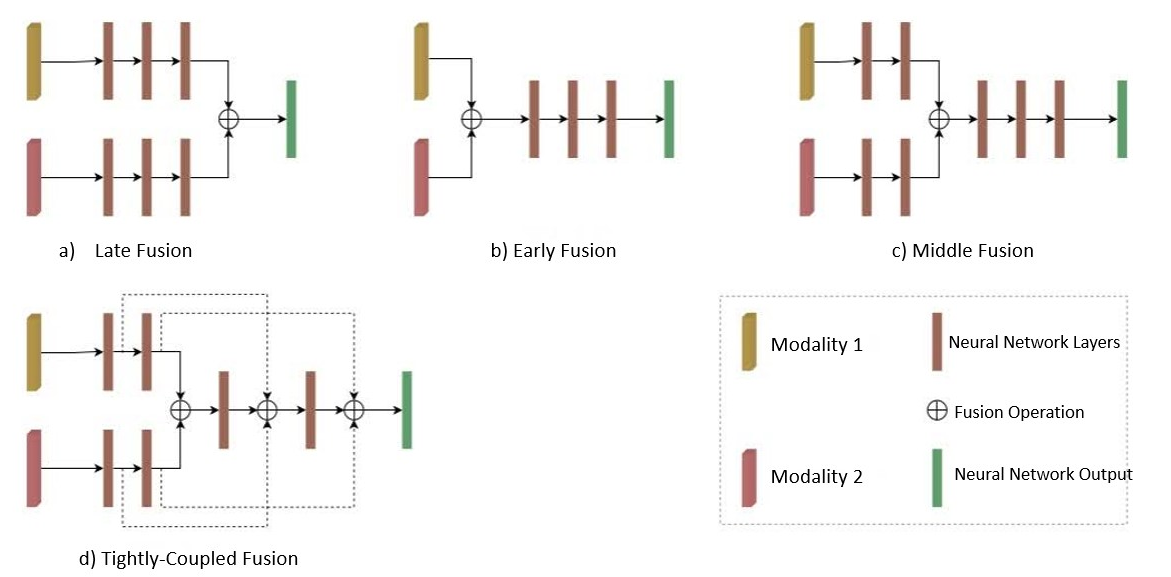
\includegraphics[width=0.8\textwidth]{images/background/emt_fusion.png}
        \caption{Different types of fusion architectures (Image adapted from \cite{yao2023radar})}
        \label{fig:fusion_types}
    \end{figure}

    \paragraph*{Early Fusion} 

    Early fusion in deep learning refers to the integration of raw or pre-processed information from modality 1 and modality 2 at the initial stages of the model. This process includes methods such as merging information from both modalities into networks for enhanced feature extraction, as well as the development of unique representations that combine elements from both sources for improved semantic analysis. Alternative approaches involve creating object proposals on one modality based on information from the other, and associating data points of one modality with the corresponding elements in the other to enrich and clarify the combined image. While this approach allows for a comprehensive utilization of the characteristics from both modalities, it also presents challenges such as susceptibility to misalignments in time or space and difficulties in correlating the distinct data forms of each modality. Accurate synchronization of the two modalities is essential for the success of early fusion \cite{yao2023radar}.

    \paragraph*{Middle Fusion}

    Middle fusion in deep learning, or feature-level fusion, merges features from two modalities at an intermediate stage. Techniques like ResNet blocks and frustum-based association are used for this. It also incorporates attention mechanisms to refine the fusion process. While it allows for the design of specific feature extractors and joint learning, it doesn't completely resolve the issue of one modality being unreliable in certain scenarios \cite{yao2023radar}.

    \paragraph*{Late Fusion}

    In Late fusion, independent objects from modality 1 and modality 2 sensors are combined at a later network stage for integrated results. The main challenge is aligning these different modalities. While this method offers flexibility, it relies on the accuracy of individual sensors and may overlook valuable intermediate features, limiting the information gained from the detection results \cite{yao2023radar}.

    \paragraph*{Tightly-Coupled Fusion}

    This is a more recent approach that uses features from both modalities and fuses at multiple level in the network stages. The model complexity increases as compared other fusion methods. In this study, we focus on Tightly-Coupled Fusion in comparison to other fusion methods. In multimodal fusion, typically one modality plays a dominant role while the other offers additional data to enhance features. Tightly-Coupled fusion leverages information from various stages, effectively preserving diverse data levels. Nonetheless, this approach requires careful consideration of each modality's significance and presents certain implementation challenges \cite{yao2023radar}.



    
    
\end{document}
